\begin{figure}
    \begin{center}
	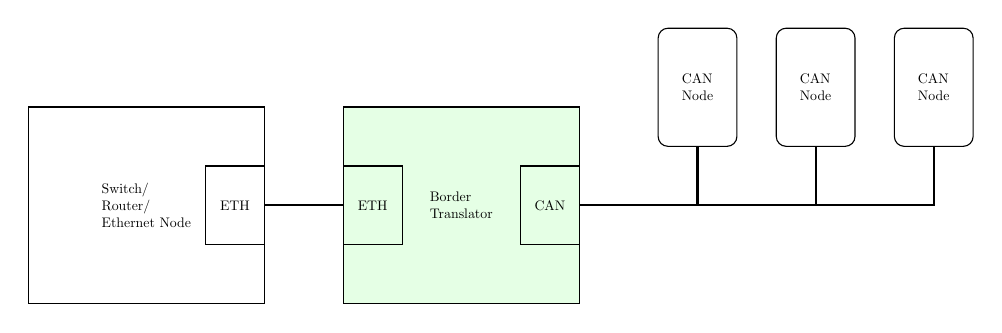
\begin{tikzpicture}[scale=0.5,  every node/.style={scale=0.5},
		rect/.style={
			draw,
			minimum height=5cm,
			minimum width=6cm,
			align=left},
			iface/.style={
			draw,
			minimum height=2cm,
			minimum width=1.5cm},
			can/.style={
			draw,
			align=left,
			minimum height=3cm,
			minimum width=2cm,
			rounded corners=0.125cm}]

		\node (switch) [rect] {Switch/ \\Router/ \\Ethernet Node};
		\node (switchEth) [iface, right of = switch, xshift=1.25cm] {ETH};

		\node (bt) [rect, fill=green!10, right of = switch, xshift=7cm] {Border \\Translator};
		\node (bteth) [iface, left of = bt, xshift=-1.25cm] {ETH};
		\node (btcan) [iface, right of = bt, xshift=1.25cm] {CAN};

		\node (can1) [can, right of = bt, xshift=5cm, yshift=3cm] {CAN \\Node};
		\node (can2) [can, right of = can1, xshift=2cm] {CAN \\Node};
		\node (can3) [can, right of = can2, xshift=2cm] {CAN \\Node};

		\draw [thick] (switchEth) -- (bteth);
		\draw [thick] (btcan) -| (can1);
		\draw [thick] (btcan) -| (can2);
		\draw [thick] (btcan) -| (can3);
	\end{tikzpicture}
	\caption{Ethernet Border Translator Schematic}
	\label{fig:bordertrans}
	\end{center}
\end{figure}